\chapter{Contracción por Bisimulación}

% \begin{definicion}
%     Sea $\model=\tup{\W,\R,\cset{\S_i}_{i \in \AGT},\V,\ACT}$ un modelo entonces se define, 
%     \begin{center}
%         $A_\modults := \{(w,v) \in \W \times \W \mid \V(w) = \V(v)\}$
%     \end{center}
%     Notar que $A_\modults$ es una relación de equivalencia sobre $\W$ (hace falta probarlo? es medio directo). Luego se denotará,
%     \begin{center}
%         $\rho_\modults := \{ [w] \mid w \in \W $ y $[w]$ su clase de equivalencia respecto a $A_\modults\}$
%     \end{center}
% \end{definicion}


% \begin{lema}
%     Sea $\model=\tup{\W,\R,\cset{\S_i}_{i \in \AGT},\V,\ACT}$ un modelo finito y sea $U \subseteq \W$ entonces,
%     \begin{center}

%     existe $S \in \mathcal{P}(\rho_\modults)$ finito tal que  $(U = \bigcup\limits_{s_i \in S} s_{i})$ \quad si y sólo si \quad $U$ es proposicionalmente definible. 
%     \end{center}
% \end{lema}

% Intuitivamente, lo que nos dice este lema es que todo conjunto proposicionalmente definible viene de tomar una cierta cantidad de clases de equivalencia de $\rho_\modults$ y unirlas. Y, a su vez, cualquier unión de una cierta cantidad de clases de equivalencia es un conjunto proposicionalmente definible. 

% Me gustaría cambiar este lema por para cada $s_i \in \rho_\modults$ se cumple que $s_i \subseteq U \vee s_i \cap U = \emptyset$ si y sólo si $U$ es proposicionalmente definible.

% Porque es una condición mucho más algorítmica, deja servido el corolario de \KHilogic-definability.



% \begin{demostracion}
%     Se demostrará por separado los casos $(\rightarrow)$ y $(\leftarrow)$.

%     Sea $\model=\tup{\W,\R,\cset{\S_i}_{i \in \AGT},\V,\ACT}$ un modelo finito y sea $U \subseteq \W$. Un primer detalle a tener en cuenta es que, dado que $\modults$ es finito, existen un número finito de variables proposicionales $p_1,...,p_n$ tales que $\{p_1,...,p_n\}$ es la imagen de $\V$.

%     \begin{itemize}
%         \item $(\rightarrow)$ Notemos primero que si $U = \emptyset$, luego la fórmula $ \varphi := \bot$ define a $U$. Entonces supongamos que $U \neq \emptyset$. (esto se podría analizar por separado o capaz permitir que S sea vacío y que en ese caso $\varphi$ sea una disyunción de 0 cosas por lo que sería el elemento neutro de la disyunción o sea $\bot$).
        
%         Sea $S = \{s_1,...,s_m\}$ finito tal que $S \in \mathcal{P}(\rho_\modults)$ y $U = \bigcup\limits_{s_i \in S} s_{i}$, demostremos que $U$ es proposicionalmente definible. 

%         Recordar que cada $s_i$ es una clase de equivalencia de la relación $A_\modults$. A su vez, para cada $w$, $v \in s_i$ se cumple que $\V(w) = \V(v)$. Se utilizará $\V(s_i)$ para hacer referencia a $\V(w)$ para cada $w \in s_i$.

%         Sea $\varphi_i := \bigwedge\limits_{j = 1}^{n} l_i(p_j)$ donde $l_i(p_j) = $
%         $\left\{ \begin{array}{rcl}
%                 p_j & \mbox{si}
%                 & p_j \in \V(s_i) \\ \neg p_j & \mbox{si} & p_i \notin \V(s_i) \\
%                 \end{array}\right.
%         $.

%         Veamos que por la forma en la que construimos $\varphi_i$, se cumple que $\modults, w \models \varphi_i$ si y sólo si $w \in s_i$. ($*$)
%         (esto podría explicarlo/demostrarlo un poco más en profundidad si no es algo claro).
        
%         Demostremos entonces que $\varphi := \bigvee\limits_{i = 1}^{m}\varphi_i$ define a $U$. Primero, notar que sea $w \in \W$, $\modults, w \models \varphi$ si y sólo si $\modults, w \models \varphi_i$ para algún $i \in \{1,...m\}$.  

%         Queremos ver entonces que, $w \in U$ si y sólo si $\modults, w \models \varphi$. 

%         Sea $w \in U$, por hipótesis, existe $s_i$ tal que $w \in s_i$. Ahora bien, por $(*)$, $\modults, w \models \varphi_i$, por lo que $\modults, w \models \varphi$.

%         Sea $w \in \W$ tal que $\modults, w \models \varphi$, entonces existe $i \in \{1,...,m\}$ tal que $\modults, w \models \varphi_i$. Luego por $(*)$, $w \in s_i$, lo que nos dice que $w \in U$.

%         Luego $\varphi$ define a $U$.
        
%         Como $\varphi$ es proposicional, $U$ es proposicionalmente definible. 
    
%         \item $(\leftarrow)$ Sea $\varphi$ la fórmula proposicional que define a $U$, se quiere demostrar que existe $S = \{s_1,...,s_m\}$ finito, tal que $S \in \mathcal{P}(\rho_\modults)$ tal que $U = \bigcup\limits_{s_i \in S} s_{i}$. 

%         Definamos $U' = \bigcup\limits_{w \in U} [w]$, siendo $[w]$ la clase de equivalencia de $w$ con respecto a $A_\modults$. Notemos que por la definición de $U'$, existe $S \in \mathcal{P}(\rho_\modults)$ finito tal que $U' = \bigcup\limits_{s_i \in S} s_{i}$ dado que $U'$ está definido como una unión finita de elementos de $\mathcal{P}(\rho_\modults)$.

%         Demostremos ahora que $U' = U$. Es claro que $U \subseteq U'$, dado que $w \in [w]$ para cada $w \in \W$.

%         Queda demostrar que $U' \subseteq U$. 
        
%         Sea $w' \in U'$, existe $w \in U$ tal que $w' \in [w]$. Ahora bien, como $w \in U$, $\modults, w \models \varphi$. Luego, notemos que por Lema 1, $\modults, v \models \varphi$ para cada $v \in [w]$, pues $\V(w) = \V(v)$ para cada $v \in [w]$.
%         Pero como $w' \in [w]$ esto nos dice que $\modults, w' \models \varphi$. Luego $w' \in U$.

%         Finalmente $U' = U$, lo cual demuestra $(\leftarrow)$.
%     \end{itemize}

% \end{demostracion}

% % IDEA PARA PROBAR LO DE QUE CADA CLASE DE EQUIVALENCIA O ESTÁ POR COMPLETO O NO ESTÁ, HABRÍA QUE PROBAR EL SII, ACÁ SOLO PRUEBO EL ->

% % \begin{corolario}
% %     Sea $\model=\tup{\W,\R,\cset{\S_i}_{i \in \AGT},\V,\ACT}$ un modelo finito y sea $U \subseteq \W$ un conjunto proposicionalmente definible, entonces
% %     \begin{center}
% %         $\forall s_i \in \rho_\modults.$ $(s_i \subseteq U \vee s_i \cap U = \emptyset)$
% %     \end{center}
% % \end{corolario}

% % \begin{demostracion}
% %     Sea $\model=\tup{\W,\R,\cset{\S_i}_{i \in \AGT},\V,\ACT}$ un modelo finito y sea $U \subseteq \W$ proposicionalmente definible.
    
% %     Supongamos que la propiedad es falsa, luego existe $s' \in \rho_\modults$ tal que $s' \nsubseteq U \wedge s_i \cap U \neq \emptyset$. Notemos que esto dice que existen $w,v \in s'$ tal que $w \in U$ y $v \notin U$.

% %     A su vez, por Lema 2, como $U$ es proposicionalmente definible existe $S \subseteq \mathcal{P}(\rho_\modults)$ tal que $U = \bigcup\limits_{s_i \in S} s_{i}$. 
    
% %     Como $w \in U$ y $w \in s'$, entonces ocurre que $s' \in S$, pues recordemos que los elementos de $\rho_\modults$ son clases de equivalencia, es decir, $s'$ es la única clase que contiene a $w$. Ahora bien, pero como $v \in s'$ entonces $v\in U$, lo cuál es absurdo, pues dijimos que $v \notin U$. 

% %     El absurdo vino de suponer que existía $s' \in \rho_\modults$ tal que  $s' \nsubseteq U \wedge s_i \cap U \neq \emptyset$, luego la propiedad queda demostrada.
% % \end{demostracion}



% \begin{corolario}
%     Sea $\model=\tup{\W,\R,\cset{\S_i}_{i \in \AGT},\V,\ACT}$ un modelo finito y sea $U \subseteq \W$ entonces el problema de decidir si $U$ es proposicionalmente definible está en $\Poly$.

%     Más aún, en caso de ser definible, encontrar una fórmula $\varphi$ que define a $U$ es realizable en tiempo polinomial en el tamaño de $\modults$.
% \end{corolario}
% (Este corolario es el problema de \KHilogic-definibilidad, porque como dijimos un conjunto es \KHilogic-definible si y sólo si es proposicionalmente definible)

% \begin{demostracion}
%     Queremos encontrar un algoritmo que dado $\model=\tup{\W,\R,\cset{\S_i}_{i \in \AGT},\V,\ACT}$ un modelo finito y $U \subseteq \W$ decida en tiempo polinomial en el tamaño de $\modults$ si $U$ es proposicionalmente definible.

%     Por Lema 2, sabemos que basta con encontrar $S \in \mathcal{P}(\rho_\modults)$ tal que $U = \bigcup\limits_{s_i \in S} s_{i}$ o determinar que no existe tal $S$.
    
%     Como $\rho_\modults$ es la partición de $\W$ con respecto a la relación de equivalencia $A_\modults$, dicho $S \in \mathcal{P}(\rho_\modults)$ existirá si y sólo si ocurre que para cada $s_i \in \rho_\modults$ se cumple que $s_i \subseteq U$ o $s_i$ $\cap$ $U = \emptyset$. (Puedo desarrollar esto acá o incluso probar un lema más que enuncie esto, pero la idea intuitiva es que como queremos chequear que U es unión de clases de equivalencia, entonces si o si tiene que ocurrir que para cada clase de equivalencia están todos sus nodos en U o ninguno está en U)

%     Entonces notemos que basta con dar un algoritmo que encuentre las clases de equivalencia de $\rho_\modults$ y para cada una de ellas chequee que, o todos sus nodos pertenecen a $U$ o ninguno de ellos lo hace.

%     % acá va algoritmo que chequea si u es definible

    


        

%     Luego, en caso de ser $U$ definible, tendremos computado ya el conjunto $S \in \mathcal{P}(\rho_\modults)$ tal que $U = \bigcup\limits_{s_i \in S} s_{i}$, que estaría formado por las clases de equivalencia que encontramos en el paso anterior que están completamente contenidas en $U$.

%     Ahora bien, a partir de dicho conjunto $S = \{s_1,...,s_m\}$, podemos computar una fórmula que define a $U$ siguiendo la misma estrategia mencionada en la demostración del Lema 2. 
    
%     Es decir, podemos computar $\varphi := \bigvee\limits_{i = 1}^{m}\varphi_i$, con $\varphi_i := \bigwedge\limits_{j = 1}^{n} l_i(p_j)$ donde $l_i(p_j) = $
%         $\left\{ \begin{array}{rcl}
%                 p_j & \mbox{si}
%                 & p_j \in \V(s_i) \\ \neg p_j & \mbox{si} & p_j \notin \V(s_i) \\
%                 \end{array}\right.
%         $.

%     Notar que la cantidad de disyunciones ($m$) de $\varphi$ está acotada por la cantidad de elementos de $\W$ y por otro lado la cantidad de conjunciones de cada término ($n$) es la cantidad de variables proposicionales que aparecen en la imagen de $\V$. Juntando estos dos argumentos, podemos deducir que el tamaño de $\varphi$ es $\bigO(|\W| *|\V|)$, lo cuál es polinomial en el tamaño de $\modults$.

%     Falta escribir el algoritmo y probar su complejidad.
% \end{demostracion}

Como hemos mencionado a lo largo de este trabajo, la noción de bisimulación nos permite relacionar modelos lógicamente equivalentes a partir de 
características estructurales entre sí. En el capítulo anterior, determinamos qué tan complejo es decidir si existe una bisimulación entre dos 
modelos.

Otra pregunta que surge a la hora de estudiar una lógica modal y su respectiva noción de bisimulación es:
Dado un modelo, ¿Existe un procedimiento capaz de encontrar otro modelo que sea bisimilar?. Más aún, ¿Podría dicho procedimiento encontrar 
un modelo de tamaño mínimo entre todos los modelos bisimilares al modelo original?.

En la lógica modal básica la respuesta a esta pregunta es positiva, y al modelo encontrado se lo llama la contracción por bisimulación.
Como se presenta en [\cite{HandbookModalLogic}, capítulo 3], la contracción se define a partir del estudio de las autobisimulaciones del modelo. En particular,
se demuestra que la unión de dos bisimulaciones es también una bisimulación, de allí se obtiene que existe una autobisimulación máxima de un modelo.

Luego, se demuestra que dicha autobisimulación máxima es una relación de equivalencia, por lo que se puede definir un modelo cuyo dominio sea el cociente
del dominio del modelo original con respecto a su autobisimulación máxima, donde cada punto representa una clase de equivalencia de dicha autobisimulación, y donde 
dos clases de equivalencia se relacionan entre sí cuando existen dos puntos de dichas clases que se relacionaban en el modelo original.

Finalmente se concluye que dicha contracción satisface que cada punto del modelo original es bisimilar al punto que representa su clase de equivalencia, y 
que, a su vez, es de tamaño mínimo entre todos los modelos bisimilares.

Habiendo mencionado un poco la ruta de trabajo seguida para la lógica modal básica, intentaremos realizar un estudio similar para la lógica `Knowing-How' basada en la 
incertidumbre.

\section{Primera Propuesta de Contracción}

\begin{definicion}
    Sea $\model=\tup{\W,\R,\cset{\S_i}_{i \in \AGT},\V,\ACT}$ un \ults, y $Z \subseteq \W \times \W$ entonces decimos que
    \begin{center}
        $Z$ es una autobisimulación de $\modults$ si y sólo si $Z$ es una \KHilogic-bisimulación        
    \end{center}
\end{definicion}

Recordemos la definición de $A_\modults$ y de $\rho_\modults$, introducida en \ref{def:Am}, y veamos el siguiente teorema 
que caracteriza la autobisimulación máxima de un modelo.

\begin{teorema}
    Sea $\model=\tup{\W,\R,\cset{\S_i}_{i \in \AGT},\V,\ACT}$ un modelo, entonces se cumple que,
    \begin{itemize}
        \item $A_\modults$ es una autobisimulación de $\modults$.
        \item Sea $Z \subseteq \W \times \W$ una autobisimulación de $\modults$ entonces $Z \subseteq A_\modults$. 
        Es decir, $A_\modults $ es la máxima autobisimulación de $\modults$. 
    \end{itemize}
\end{teorema}

\begin{demostracion}
    Sea $\model=\tup{\W,\R,\cset{\S_i}_{i \in \AGT},\V,\ACT}$ un \ults, probaremos ambas propiedades por separado:

    \begin{itemize}
        \item Queremos ver que $A_\modults$ es una autobisimulación de $\modults$, para ello debemos verificar que:
        \begin{itemize}
            \item (Atom) Dado $(w,v) \in A_\modults$, por definición de $A_\modults$, se cumple que $\V(w) = \V(v)$.
            \item (A-Zig) Notemos que $A_\modults$ es una relación de equivalencia, luego para cada $w\in \W$ se cumple que $(w,w) \in A_\modults$.
            \item (A-zag) Podemos utilizar el mismo argumento que en (A-zig) para demostrar este caso.
            \item ($\khi$-zig) Sea $U \subseteq \W$ tal que para cada $s_i \in \rho_\modults$ se cumple que $s_i \cap U = \emptyset$ o 
            $s_i \subseteq U$, si $U \ultsExecAgi T$ para algún $T \subseteq \W$, entonces existe $T' \subseteq \W$ tal que
                \begin{multicols}{2}
                    \begin{itemize}
                        \item $A_\modults(U) \ultsExecAgi T'$, 
                        \item $T' \subseteq A_\modults(T)$.
                    \end{itemize}
                \end{multicols}

            Sean $U,T$ subconjuntos de $\W$ tales que $U \ultsExecAgi T$ y $U$ es tal que para cada $s_i \in \rho_\modults$ se cumple que 
            $s_i \cap U = \emptyset$ o $s_i \subseteq U$, queremos encontrar $T' \subseteq \W$ que cumpla lo mencionado.
            
            Demostremos por un lado que $U = A_\modults(U)$:
            
            ($\subseteq$) Siguiendo el argumento usado en (A-Zig), es claro que para $w \in U$ se cumple que $w \in A_\modults(U)$, 
            pues $(w,w) \in A_\modults$ para cada $w \in \W$. 
            
            ($\supseteq$) Sea $v \in A_\modults(U)$, queremos ver que $v \in U$.
            Como $v \in A_\modults(U)$, entonces existe $w \in U$ tal que $(w,v) \in A_\modults$ y, por lo tanto, $v \in [w]$.
            
            Como $w \in U$ entonces $[w] \subseteq U$. Luego $v \in U$.

            Entonces demostramos que $U = A_\modults(U)$.

            Notemos que siendo $X \subseteq \W$ entonces $X \subseteq A_\modults(X)$, pues como analizamos anteriormente 
            $(w,w) \in A_\modults$ para cada $w \in \W$.

            Juntando lo mencionado, podemos afirmar que $T' = T$ cumple que:

             \begin{itemize}
                \item $A_\modults(U) \ultsExecAgi T'$, pues dijimos $A_\modults(U) = U$, y por hipótesis, $U \ultsExecAgi T = T'$.  
                \item $T' \subseteq A_\modults(T')$ pues esto se cumple para todo $X \subseteq \W$.
            \end{itemize}
            Luego queda demostrado que $A_\modults$ satisface ($\khi$-zig).

            \item ($\khi$-zag) Análogo a ($\khi$-zig), pues notemos que como $A_\modults$ es una relación de equivalencia, es simétrica.
        \end{itemize}

        Luego $A_\modults$ es una autobisimulación de $\modults$.
        
        \item Queremos ver que dada $Z \subseteq \W \times \W$ autobisimulación de $\modults$, entonces $Z \subseteq A_\modults$.
        
        Supongamos que no es cierto, es decir, existe $Z \subseteq \W \times \W$ autobisimulación de $\modults$ tal que hay 
        $w,v \in \W$ que cumplen que $(w,v) \in Z$ y $(w,v) \notin A_\modults$. 

        Como $Z$ es una autobisimulación entonces satisface (Atom), es decir, $\V(w) = \V(v)$. Pero notemos que por definición de 
        $A_\modults$, $(w,v) \in A_\modults$, lo cuál es absurdo, pues dijimos que $(w,v) \notin A_\modults$.

        El absurdo vino de suponer que $Z \nsubseteq A_\modults$.    
    \end{itemize}
    Luego queda demostrada la propiedad.
\end{demostracion}

Una primera observación que surge a partir de este teorema es que, a diferencia de lo mencionado sobre el caso de la lógica modal básica, 
encontramos una forma de identificar la autobisimulación máxima de un modelo sin necesidad de demostrar que la unión preserva bisimulación. 

En particular, se demuestra que la partición de nodos de acuerdo a la función de valuación $\V$ siempre es una autobisimulación.

Entonces sea $\modults$ un \ults, nos gustaría definir su contracción por bisimulación a partir de $A_\modults$ su autobisimulación máxima.

Tomando un camino similar al de la lógica modal básica, una posible primer propuesta sería un modelo en el que se tenga como dominio al cociente 
de $\modults$ con respecto a $A_\modults$ y se relacione a las clases de equivalencia $[w], [v] \in \rho_\modults$ siempre que 
$w, v$ estén relacionados en $\modults$. Por otro lado, la relación de indistinguibilidad de cada agente y el conjunto de acciones de $\modults$ se conservarían.

Sin embargo consideremos el siguiente modelo (\Cref{fig:1stproposaloriginal}):

\begin{figure}[h]
    \centering
    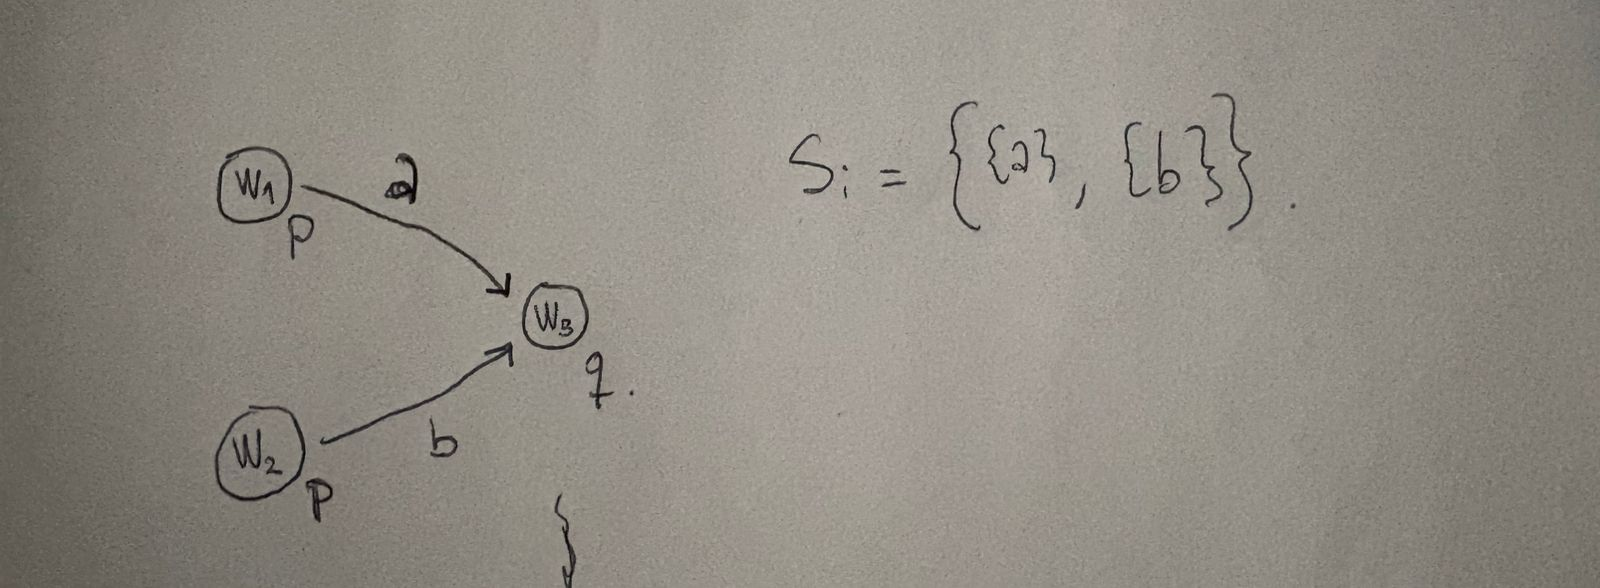
\includegraphics[width=0.5\textwidth]{imagenes/1ra_propuesta_original.jpeg}
    \caption{$\modults$}
    \label{fig:1stproposaloriginal}
\end{figure}

Con esta propuesta de contracción ($\modults'$), obtendríamos el modelo (\Cref{fig:1stproposalcontraction}):

\begin{figure}[h]
    \centering
    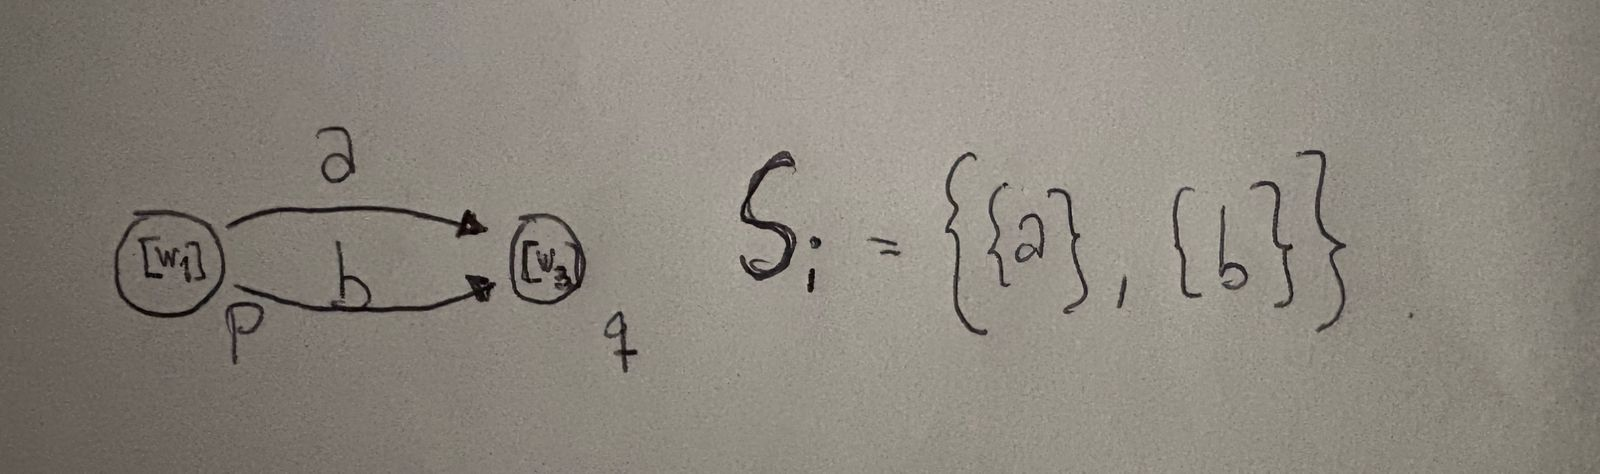
\includegraphics[width=0.5\textwidth]{imagenes/1ra_propuesta_contraido.jpeg}
    \caption{$\modults'$}
    \label{fig:1stproposalcontraction}
\end{figure}


Notemos que $\modults, w_1 \not\models \khi(p,q)$ pero $\modults', [w_1] \models \khi(p,q)$, luego $\modults,w_1$ y 
$\modults',[w_1]$ no son bisimilares.

Por lo que esta contracción por bisimulación no sería adecuada, ya que no produce un modelo bisimilar al modelo original.

Otra posible propuesta sería restringir más la relación entre las puntos del modelo contraído. Es decir, relacionar las clases 
$[w], [v] \in \rho_\modults$ cuando para cada $w' \in [w]$ existe $v' \in [v]$ tal que $w'$ y $v'$ están relacionados en el modelo original.

Luego consideremos el siguiente modelo (\Cref{fig:2ndproposaloriginal}):

\begin{figure}[h]
    \centering
    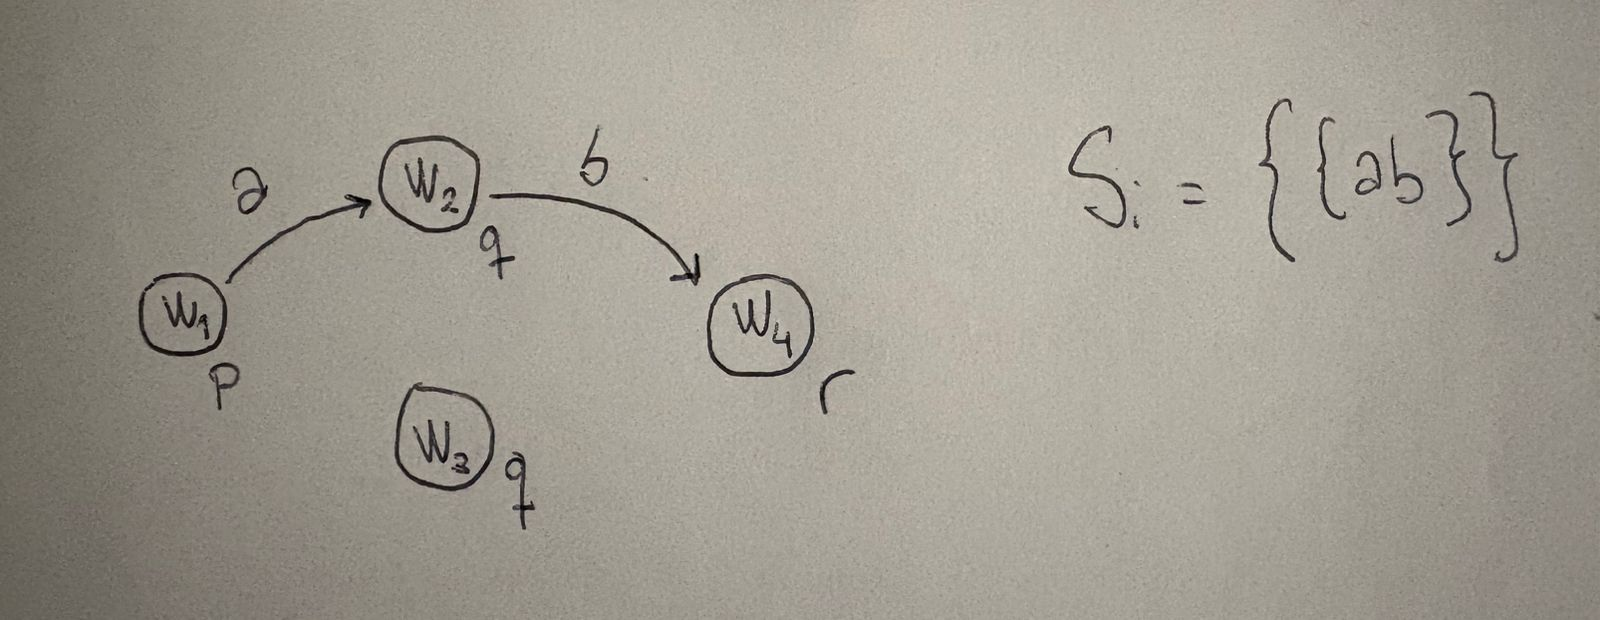
\includegraphics[width=0.5\textwidth]{imagenes/2da_propuesta_original.jpeg}
    \caption{$\modults$}
    \label{fig:2ndproposaloriginal}
\end{figure}

Y su contracción por bisimulación con la propuesta mencionada (\Cref{fig:2ndproposalcontraction}):

\begin{figure}[h]
    \centering
    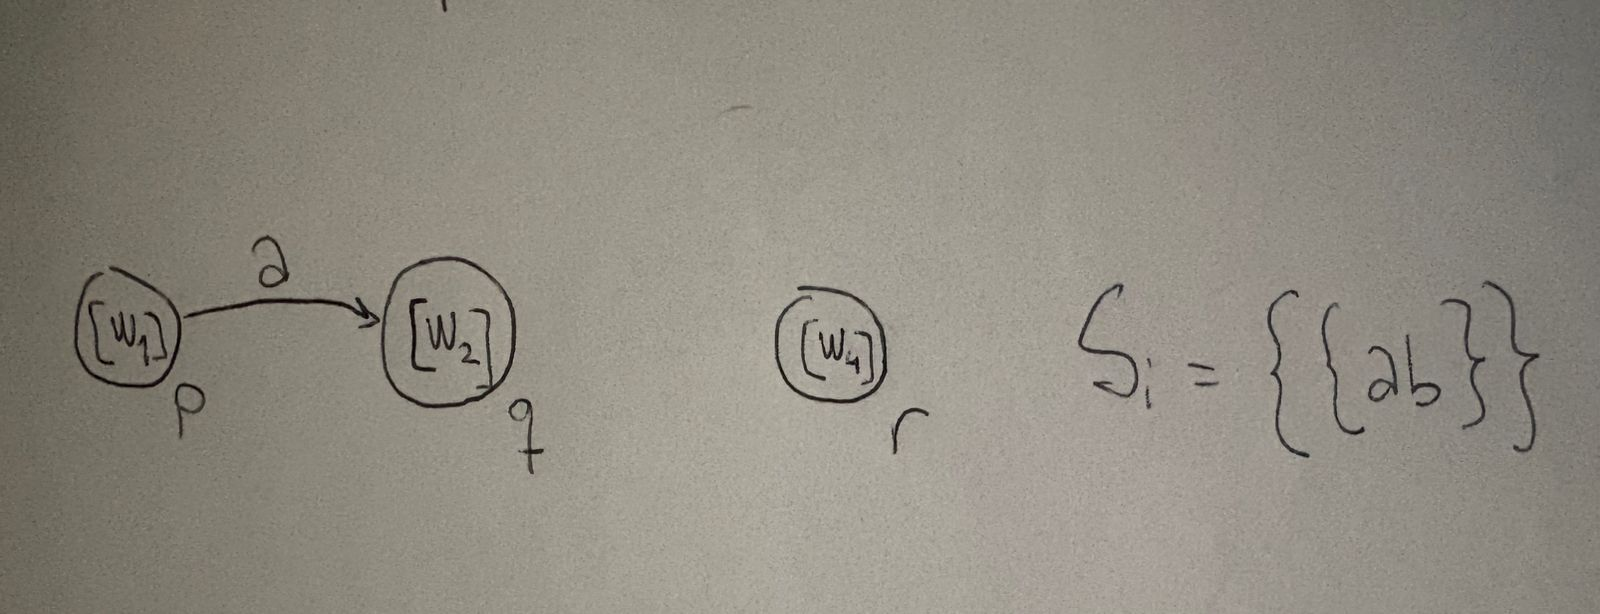
\includegraphics[width=0.5\textwidth]{imagenes/2da_propuesta_contraido.jpeg}
    \caption{$\modults'$}
    \label{fig:2ndproposalcontraction}
\end{figure}

Si analizamos ambos modelos, podemos notar que $\modults,w_1 \models \khi(p,r)$ pero $\modults',[w_1] \not\models \khi(p,r)$, luego 
$\modults,w_1$ y $\modults',[w_1]$ no son bisimilares.

Por lo que esta propuesta tampoco es adecuada, ya que tampoco produce un modelo bisimilar al modelo original.

Si analizamos ambos contraejemplos, podemos notar que la primera propuesta de contracción podría agregar caminos fuertemente ejecutables al modelo 
y la segunda podría eliminar caminos fuertemente ejecutables del modelo. Los fallos de ambas propuestas nos dan la idea de que no parece 
existir una contracción directa en la cuál no se modifique la relación de indistinguibilidad de cada agente y las acciones 
consideradas por el modelo. 

A partir de lo mencionado, surge la siguiente propuesta de contracción, la cuál modifica el conjunto de acciones y la relación de indistinguibilidad 
de cada agente.


\begin{definicion}
    Sea $\model=\tup{\W,\R,\cset{\S_i}_{i \in \AGT},\V,\ACT}$ un \ults. Se define su contracción por bisimulación, $\model'=\tup{\W',\R',\cset{\S_i'}_{i \in \AGT'},\V',\ACT'}$ donde 
    \begin{center}
        \begin{itemize}
            \item $\W' := \W/A_\modults$
            \item $\R' := \{\R'_{a_\sigma} \subseteq \W' \times \W' \mid a_\sigma \in \ACT'\}$ donde $([w],[v]) \in \R'_{a_\sigma}$ si y sólo si
            \begin{enumerate}
                \item existen $w' \in [w]$ y $v' \in [v]$ tal que $(w',v')\in \R_\sigma$
                \item $\sigma$ es fuertemente ejecutable para cada $w' \in [w]$.
            \end{enumerate}
            \item $\S_i' := \{ \pi' = \{a_\sigma \mid \sigma \in \pi\} \mid \pi \in S_i \}$
            \item $\V'([w]) := \V(w)$
            \item $\ACT' := \{a_\sigma \mid $ existe $ \pi\in S_i$ tal que $ \sigma \in \pi$ para algún $i \in \AGT \}$ 
        \end{itemize}
    \end{center}
\end{definicion}
    
Una vez presentada la contracción, demostraremos que produce un modelo bisimilar. Para ello demostraremos el siguiente teorema.

\begin{teorema}
    Sea $\model=\tup{\W,\R,\cset{\S_i}_{i \in \AGT},\V,\ACT}$ un \ults y sea $\modults'$ su contracción por bisimulación entonces 
    $\tup{\modults,w}$ y $\tup{\modults',[w]}$ son $\KHilogic$-bisimilares para cada $w \in \W$.
\end{teorema}

\begin{demostracion}
    Sea $\model=\tup{\W,\R,\cset{\S_i}_{i \in \AGT},\V,\ACT}$ un \ults
    y sea $\modults'$ su contracción por bisimulación, basta ver que $Z = \{(w,[w]) \in \W \times\W'\}$ es una \KHilogic-bisimulación para demostrar la propiedad.

    Dado que $\W$ es no vacío entonces es claro que $Z$ es no vacío también.

    Por otro lado, notemos que por la definición de $\V'$, es claro que $Z$ satisface (Atom).

    A su vez, por cómo definimos $Z$, es fácil ver que también (A-zig) y (A-zag) son satisfechos.
    
    Demostremos entonces que se satisfacen ($\khi$-zig) y ($\khi$-zag).

    \begin{itemize}
        \item ($\khi$-zig) Sean $U, T$ subconjuntos de $\W$ tales que $U \ultsExecAgi T$ y para cada $s \in \rho_\modults$ se cumple que 
        $s \subseteq U$ o $s \cap U = \emptyset$, queremos encontrar $T' \subseteq \W'$ que

        \begin{multicols}{2}
            \begin{itemize}
                \item $Z(U) \ultsExecAgi T'$, 
                \item $T' \subseteq Z(T)$.
            \end{itemize}
        \end{multicols}

        Veamos que $T' := \{ [w] \mid w \in T\}$ cumple con lo mencionado. Por como definimos $Z$, es claro que $T'  = Z(T)$, por lo que 
        $T' \subseteq Z(T)$. Entonces demostremos $Z(U) \ultsExecAgi T'$.

        Como $U \ultsExecAgi T$, existe $\pi \in S_i$ tal que cada plan de $\pi$ es fuertemente ejecutable en cada nodo de $U$ y 
        $\R_\pi(U) \subseteq T$. 

        Sabemos por la definición de $\modults'$ que existe $\pi' = \{a_\sigma \mid \sigma \in \pi\} \in S_i'$. Demostraremos que $\pi'$ 
        atestigua $Z(U) \ultsExecAgi T'$, es decir, que cada $a_\sigma \in \pi$ es fuertemente ejecutable en $Z(U)$ y que además 
        $\R'_{\pi'}(Z(U)) \subseteq T'$.

        Sea $[w] \in Z(U)$, veamos que $\pi'$ es fuertemente ejecutable en $[w]$. Sea $a_\sigma \in \pi'$, queremos ver que $a_\sigma$ es fuertemente 
        ejecutable en $[w]$. Notar que cómo $a_\sigma$ es un plan de un solo paso, solo basta con ver que exista $[v] \in \W'$  tal que 
        $([w],[v]) \in \R'_{a_\sigma}$.
        
        Primero notemos que como $[w] \in Z(U)$, entonces existe $w' \in [w]$ tal que $w' \in U$. Luego, por la hipótesis sobre $U$
        se cumple que $[w'] = [w] \subseteq U$. Pero veamos que como $\pi$ es fuertemente ejecutable en $U$ entonces es fuertemente ejecutable en cada nodo 
        de $[w]$, por lo que existe $v' \in \W$ tal que $v \in \R_\sigma(w')$. Como $\sigma$ es fuertemente en todo $[w]$ y $(w',v') \in \R_\sigma$, entonces 
        $([w],[v']) \in \R'_{a_\sigma}$. Queda demostrado entonces que $\pi'$ es fuertemente ejecutable en $Z(U)$.
        
        Demostraremos ahora que $\R'_{\pi'}(Z(U)) \subseteq T'$.

        Sea $[v] \in \R'_{\pi'}(Z(U))$, entonces existe $[w] \in Z(U)$ y $a_\sigma \in \pi'$ tal que $([w],[v]) \in \R'_{a_\sigma}$. Notar que 
        como $[w] \in Z(U)$, entonces existe $w' \in [w]$ tal que $w' \in U$ y, por lo tanto, $[w'] = [w] \subseteq U$. Si analizamos la definición 
        de $\R'_{a_\sigma}$, como $([w],[v]) \in \R'_{a_\sigma}$ entonces existen $w'' \in [w]$ y $v'' \in [v]$ tal que $(w'',v'') \in \R_\sigma$.
        Como $w'' \in U$ y $\R_\pi(U) \subseteq T$, entonces se cumple que $v'' \in T$, lo que nos dice que $[v''] = [v] \in T'$, que era lo que 
        queríamos demostrar. Luego $\R'_{\pi'}(Z(U)) \subseteq T'$. 

        Queda demostrado entonces $Z$ satisface $\khi$-zig.

        \item ($\khi$-zag) Sean $U', T' \in \W'$ tales que $U' \ultsExecAgi T'$ y para cada $s \in \rho_{\modults'}$ se cumple que $s \subseteq U'$ o 
        $s \cap U' = \emptyset$, queremos encontrar $T \subseteq \W$ tal que:
        \begin{multicols}{2}
            \begin{itemize}
                \item $Z^{-1}(U') \ultsExecAgi T$, 
                \item $T \subseteq Z^{-1}(T')$.
            \end{itemize}
        \end{multicols}
        
        Veamos que $T := \bigcup\limits_{[w] \in T'} [w]$ cumple con lo mencionado. Notar que por la definición de $Z$, es claro que $T' = Z^{-1}(T)$, lo que nos dice que $T' \subseteq Z^{-1}(T)$. Demostremos entonces que $Z^{-1}(U) \ultsExecAgi T'$. 
    
        Como $U' \ultsExecAgi T'$, entonces existe $\pi' \in S_i'$ tal que $\pi'$ es fuertemente ejecutable para cada $[w] \in U'$ y $\R'_{\pi'}(U') \subseteq T'$.

        Luego, por como está definido $\modults$ existe $\pi \in S_i$ tal que para cada $\sigma \in \pi$, $a_\sigma \in \pi'$. 
        Veamos entonces que $\pi$ atestigua $Z^{-1}(U') \ultsExecAgi T$, es decir, que $\pi$ es fuertemente ejecutable para cada $w \in Z^{-1}(U')$ 
        y, a su vez, que $\R_\pi(Z^{-1}(U')) \subseteq T$.

        Sean $w \in Z^{-1}(U')$, veamos que $\pi$ es fuertemente ejecutable en $w$. Sea $\sigma \in \pi$, veamos que $\sigma$ es fuertemente ejecutable 
        en $w$. Notemos que como $w \in Z^{-1}(U')$ entonces $[w] \in U'$ y, a su vez, como $a_\sigma$ es fuertemente ejecutable en $U'$, $a_{\sigma_i}$ también es fuertemente ejecutable en $[w]$. 
        Luego, existe $[v]$ tal que $([w],[v]) \in \R'_{a_\sigma}$. Notemos que por la definición de $\R'$, como existe esa arista entonces se cumple que $\sigma$ es fuertemente ejecutable 
        para cada nodo de $[w]$. En particular, $\sigma$ es fuertemente ejecutable en $w$, lo que demuestra que $\pi$ es fuertemente ejecutable 
        en $Z^{-1}(U')$.

        Demostremos ahora que $\R_{\pi}(Z^{-1}(U')) \subseteq T'$. 

        Sean $w, v \in \W$ tales que $w \in Z^{-1}(U')$ y $(w,v) \in \R_\pi$, queremos ver que $v \in T'$. Primero veamos que como $(w,v) \in \R_\pi$, 
        entonces existe $\sigma \in \pi$ tal que $(w,v) \in \R_\sigma$. Luego, como $w \in Z^{-1}(U')$, entonces $[w] \in U'$. Como $\pi'$ es fuertemente 
        ejecutable en $U'$, entonces $a_\sigma$ es fuertemente ejecutable en $U'$ y por lo tanto $a_\sigma$ también es fuertemente ejecutable en $[w]$.
        
        Pero, como $a_\sigma$ es fuertemente ejecutable en $[w]$ entonces existe $[v']$ tal que $([w],[v']) \in \R_{a_\sigma}$. 
        Como existe dicha arista, por la definición de $\R'$, ocurre que $\sigma$ es fuertemente ejecutable en todo nodo de $[w]$. 
        Pero como $\sigma$ es fuertemente ejecutable en todo nodo de $[w]$ y $(w,v) \in \R_\sigma$ entonces $([w],[v]) \in \R'_{a_\sigma}$. 
        Luego, como $\R'_{\pi'}(U') \subseteq T'$, entonces $[v] \in T'$, lo que nos dice que $v \in T$ que era lo que queríamos demostrar.

        Entonces, hemos demostrado que $Z$ satisface $\khi$-zag.
    \end{itemize}
    Demostramos que $Z$ es una \KHilogic-bisimulación. Luego $\tup{\modults,w}$ y $\tup{\modults',[w]}$ son $\KHilogic$-bisimilares para cada $w \in \W$.
\end{demostracion}



\begin{teorema}
    La contracción por bisimulación de un \ults $\modults$ tiene cardinalidad mínima entre los modelos $\KHilogic$-bisimilares a $\modults$.
\end{teorema}


\begin{teorema}
    Sea $\modults$ un \ults, computar su contracción por bisimulación $\modults'$ es realizable en tiempo polinomial en el 
    tamaño de $\modults$.
\end{teorema}


\section{Segunda Propuesta de Contracción}

\begin{definicion}
    Supongamos $\ACT$ un conjunto de acciones no vacío enumerable.
    Sea $\modults = \tup{\W,\{\R_a\}_{a\in\ACT},\V}$ un modelo de Kripke. Sea $Z_\modults$ su autobisimulación máxima en Lógica Modal Básica (LMB) entonces definimos su contracción por LMB-bisimulación como $\modults_{LMB} = \tup{\W',\{\R'_a\}_{a\in\ACT},\V'}$ donde
    \begin{center}
        \begin{itemize}
            \item $\W' := \W /Z_\modults$
            \item $\R_a' := \{([w],[v]) \mid$ existen $w' \in [w]$ y $v' \in [v]$ tal que $(w',v') \in \R_a \}$
            \item $\V'([w]) := \V(w)$
        \end{itemize}
    \end{center} 
\end{definicion}

Notar que en el contexto de esta definición, $[w]$ se refiere a la clase de equivalencia de $w$ en la relación de equivalencia dada por $Z_\modults$. 


\begin{lema}
    Sea $\model = \tup{\W,\{\R_a\}_{a\in\ACT},\V}$ un modelo de Kripke, y sea $\modults_{LMB} = \tup{\W',\{\R_a'\}_{a\in\ACT},\V'}$ su contracción por LMB-bisimulación.
    Si $([w],[v]) \in \R'_a$ entonces para cada $w' \in [w]$ existe $v' \in [v]$ tal que $(w',v') \in \R_a$
\end{lema}



\begin{demostracion}
    Sea $\model = \tup{\W,\{\R_a\}_{a\in\ACT},\V}$ un modelo de Kripke, y sea $\modults_{LMB} = \tup{\W',\{\R_a'\}_{a\in\ACT},\V'}$ su contracción por LMB-bisimulación. Sea $([w],[v]) \in \R'_a$, veamos que para cada $w' \in [w]$ existe $v' \in [v]$ tal que $(w',v') \in \R_a$.

    Como $([w],[v]) \in \R'_a$ existen $w_0 \in [w]$ y $v_0 \in [v]$ tales que $(w_0,v_0)\in \R_a$. Sea $w' \in [w]$, por estar ambos 
    $w_0$ y $w'$ en $[w]$, existe una LMB-bisimulación $Z$ tal que $(w_0,w') \in Z$. Pero notemos que, por (zig) de $Z$, como 
    $(w_0,v_0) \in \R_a$  entonces existe $v'$ tal que $(w',v') \in \R_a$ y, a su vez, 
    $(v_0,v') \in Z$, es decir, $v' \in [v]$. Como demostramos esto para un $w'$ arbitrario en $[w]$, vale para todo elemento de $[w]$.
\end{demostracion}


\begin{teorema}
    Sea $\model=\tup{\W,\R,\cset{\S_i}_{i \in \AGT},\V,\ACT}$ un \ults y $\modults_{LMB} = \tup{\W',\{\R_a'\}_{a\in\ACT},\V'}$ 
    la contracción por LMB-bisimulación del modelo $\tup{\W,\{\R_a\}_{a\in\ACT},\V}$, entonces $\tup{\modults,w}$ y $\tup{\modults',[w]}$ 
    son $\KHilogic$-bisimilares para cada $w \in \W$ siendo $\modults' = \tup{\W',\R',\cset{\S_i}_{i \in \AGT},\V',\ACT}$.
\end{teorema}

Notar que en este teorema, al fijar $\model=\tup{\W,\R,\cset{\S_i}_{i \in \AGT},\V,\ACT}$ inmediatamente fijamos a $\ACT$ como el conjunto no vacío enumerable de acciones para la Lógica Modal Básica.

\begin{demostracion}
    Queremos ver que $Z = \{(w,[w]) \mid w \in \W\}$ es una \KHilogic-bisimulación.
    
    Por definición de la contracción por bisimulación en (LMB) se puede ver que se satisface (Atom). Luego, por definición de Z, es fácil ver que (A-zig) y (A-zag) son satisfechas. Demostremos entonces ($\khi$-zig) y ($\khi$-zag).

    \begin{itemize}
        \item ($\khi$-zig). Sean $U, T$ ambos subconjuntos de $\W$ tales que $U$ es proposicionalmente definible y $U \ultsExecAgi T$. Queremos ver que existe $T' \subseteq \W'$ tal que

        \begin{multicols}{2}
            \begin{itemize}
                \item $Z(U) \ultsExecAgi T'$, 
                \item $T' \subseteq Z(T)$.
            \end{itemize}
        \end{multicols}
        Veamos que $T' = \{[w] \mid w \in T\}$ cumple con lo mencionado. Notemos que $T' = Z(T)$, por lo que solo debemos demostrar $Z(U) \ultsExecAgi T'$.

        Como $U \ultsExecAgi T$, existe $\pi \in S_i$ tal que $\pi$ es fuertemente ejecutable en $U$ y a su vez $\R_\pi(U) \subseteq T$.

        Demostremos que $\pi$ es fuertemente ejecutable en $Z(U)$ y que $\R'_\pi(Z(U)) \subseteq T'$.

        Supongamos que $\pi$ no es fuertemente ejecutable en $Z(U)$. Luego existe $\sigma \in \pi$ y $[w_1],...,[w_k]$ con $0 \le k \le |\sigma|$ tal que $[w_1] \in Z(U)$, $([w_i], [w_{i+1}]) \in \R'_{\sigma[i]}$ y $\R'_{\sigma[k]}([w_k]) = \emptyset$.

        Como $[w_1] \in Z(U)$, existe $w_1' \in U$ tal que $w_1' \in [w_1]$. Luego notemos que aplicando sucesivamente el Lema 3 en todo el camino, existen $w_1',...w_k'$ tales que $w_i' \in [w_i]$ y $(w_i',w_{i+1}') \in \R_{\sigma[i]}$.

        Pero veamos que esto nos dice que $\R_{\sigma[k]}(w_k') = \emptyset$. Pues, si existiera $v$ tal que $(w_k',v) \in \R_{\sigma[k]}$ entonces ocurriría que $([w_k],[v]) \in \R'_{\sigma[k]}$. Luego $\sigma \in \pi$ no es fuertemente ejecutable en $w_1' \in U$, lo cuál es absurdo, pues dijimos que $\pi$ es fuertemente ejecutable en todo $U$.

        Esto nos dice que $\pi$ es fuertemente ejecutable en $Z(U)$.

        Veamos ahora que $\R'_\pi(Z(U)) \subseteq T'$.

        Sea $[v] \in \R'_\pi(Z(U))$, entonces existen $\sigma \in \pi$ y $[w_1], ..., [w_{|\sigma|+1}]$ tales que $[w_1] \in Z(U)$, $([w_i],[w_{i+1}]) \in \R'_{\sigma[i]}$ y $[w_{|\sigma|+1}] = [v]$.

        Como $[w_1] \in Z(U)$, entonces existe $w_1' \in U$ tal que $w_1'\in [w_1]$. Luego notemos que aplicando sucesivamente el Lema 3 sobre el camino, existen $w_1',...,w_{|\sigma|+1}'$ tales que $w_i' \in [w_i]$ y $(w_i',w_{i+1}')\in \R_{\sigma[i]}$. Como $\R_\pi(U) \subseteq T$ esto nos dice que $w'_{|\sigma|+1} \in T$. Finalmente, por definición de $T'$, $[w_{|\sigma|+1}] \in T'$. Luego como $[v] = [w_{|\sigma|+1}]$, $[v] \in T'$.

        Entonces demostramos que $\pi$ es fuertemente ejecutable en $Z(U)$ y que $\R'_\pi(Z(U)) \subseteq T'$. Juntando ambos resultados, concluimos que $Z(U) \ultsExecAgi T'$, lo cuál demuestra ($\khi$-zig).

       \item ($\khi$-zag) Sean $U,T$ ambos subconjuntos de $\W'$ tales que $U$ es proposicionalmente definible y $U \ultsExecAgi T$. Queremos ver que existe $T' \subseteq \W$ tal que

       \begin{multicols}{2}
            \begin{itemize}
                \item $Z^{-1}(U) \ultsExecAgi T'$, 
                \item $T' \subseteq Z^{-1}(T)$.
            \end{itemize}
        \end{multicols}

        Veamos que $T' = \{w \mid [w] \in T\}$ cumple con lo mencionado. Notemos que $T' = Z^{-1}(T)$ por lo que solo debemos demostrar $Z^{-1}(U) \ultsExecAgi T'$.

        Como $U \ultsExecAgi T$, existe $\pi \in S_i$ tal que $\pi$ es fuertemente ejecutable en todo $U$ y a su vez $\R'_\pi(U) \subseteq T$.

        Veamos que $\pi$ es fuertemente ejecutable en $Z^{-1}(U)$ y que $\R_\pi(Z^{-1}(U)) \subseteq T'$.

        Supongamos que $\pi$ no es fuertemente ejecutable en $Z^{-1}(U)$. Luego existe $\sigma \in \pi$ y $w_1,...,w_k$ con $0 \le k \le |\sigma|$ tal que $w_1 \in Z^{-1}(U)$, $(w_i,w_{i+1}) \in \R_{\sigma[i]}$ y $\R_{\sigma[k]}(w_k) = \emptyset$. 

        Notemos entonces que por la definición de $\R'$, $[w_1],...,[w_k]$ cumple que $([w_i],[w_{i+1}]) \in \R'_{\sigma[i]}$ y, a su vez, que $[w_1] \in U$, pues $w_1 \in Z^{-1}(U)$. Pero notemos que como $\R_{\sigma[k]}(w_k) = \emptyset$, por la contrarrecíproca del Lema 3, podemos ver que $\R'_{\sigma[k]}([w_k]) = \emptyset$, lo que nos dice que $\sigma \in \pi$ no es fuertemente ejecutable en $[w_1] \in U$. Absurdo, pues dijimos que $\pi$ es fuertemente ejecutable en todo $U$.

        Esto nos dice que $\pi$ es fuertemente ejecutable en todo $Z^{-1}(U)$.

        Veamos ahora que $\R_\pi(Z^{-1}(U)) \subseteq T'$.

        Sea $v \in \R_\pi(Z^{-1}(U))$, entonces existen $\sigma \in \pi$ y $w_1,...,w_{|\sigma|+1}$ tales que $w_1 \in Z^{-1}(U)$, $(w_i,w_{i+1}) \in \R_{\sigma[i]}$ y $w_{|\sigma|+1} = v$. 

        Por la definición de $\R'$, esto nos dice que $[w_1],...,[w_{|\sigma|+1}]$ cumple que $([w_i],[w_{i+1}]) \in \R'_{\sigma[i]}$ y, a su vez, como $w_1 \in Z^{-1}(U)$ entonces $[w_1] \in U$. Luego notemos que como $\R'_\pi(U) \subseteq T$, esto nos dice que $[w_{|\sigma|+1}] \in T$, lo cuál implica que $w_{|\sigma|+1} \in T'$. Como $v = w_{|\sigma|+1}$ entonces $v \in T'$. 

        Entonces demostramos que $\pi$ es fuertemente ejecutable en todo $Z^{-1}(U)$ y que $\R'_\pi(Z^{-1}(U)) \subseteq T'$. Juntando ambos resultados, concluimos que $Z^{-1}(U) \ultsExecAgi T'$, lo cuál demuestra ($\khi$-zag).
    \end{itemize}
    Demostramos entonces que $Z$ es una \KHilogic-bisimulación. Luego $\tup{\modults,w}$ y $\tup{\modults',[w]}$ son $\KHilogic$-bisimilares para cada $w \in \W$.
\end{demostracion}

\section{Comparación entre las contracciones propuestas}